\afterpage{
\clearpage
\begin{figure}[p]
    \centering
    \begin{subfigure}[b]{0.47\textwidth}
        \centering
        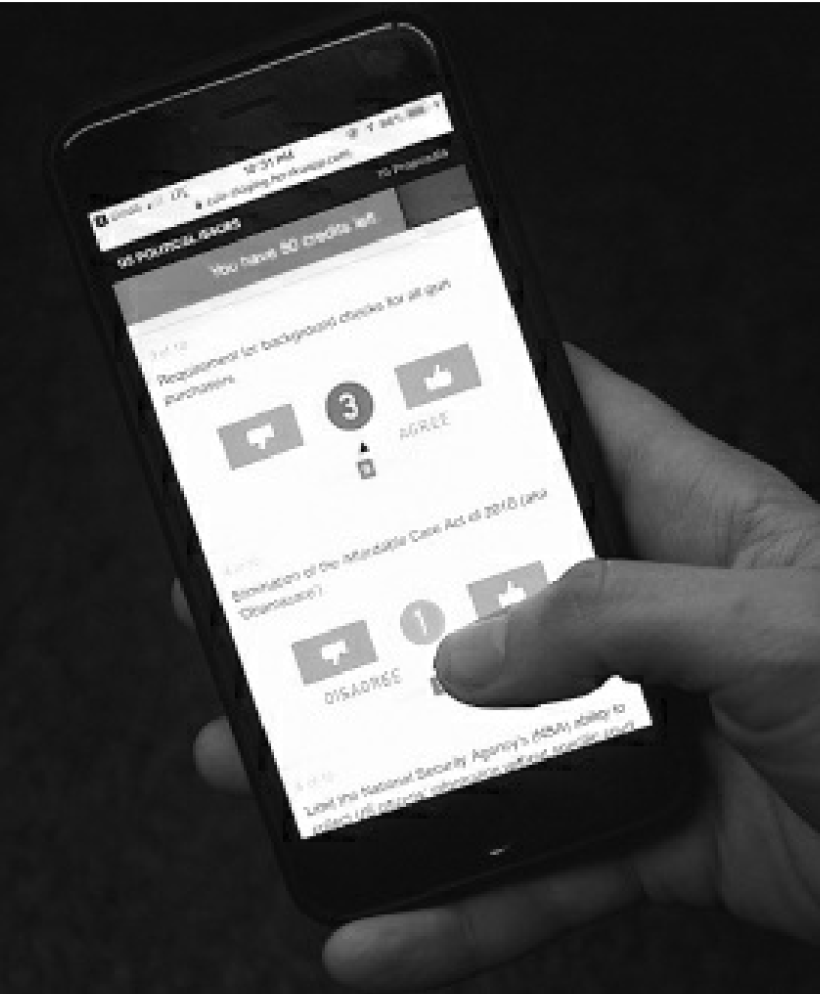
\includegraphics[width=0.67\textwidth]{content/image/curr_interface/radical_market_wedesign.png}
        \caption{Software by WeDesign, used in the first empirical QV research~\cite{quarfoot2017quadratic}. Little information is available about the software, except for an image from~\textcite{posner2018radical}. In the image, each prompt has thumbs up and down icons to update the vote in the center. The remaining budget appears as a progress bar at the top.}
        \label{fig:wedesignInterface}
    \end{subfigure}
    \hspace{0.4cm}
    \begin{subfigure}[b]{0.47\textwidth}
        \centering
        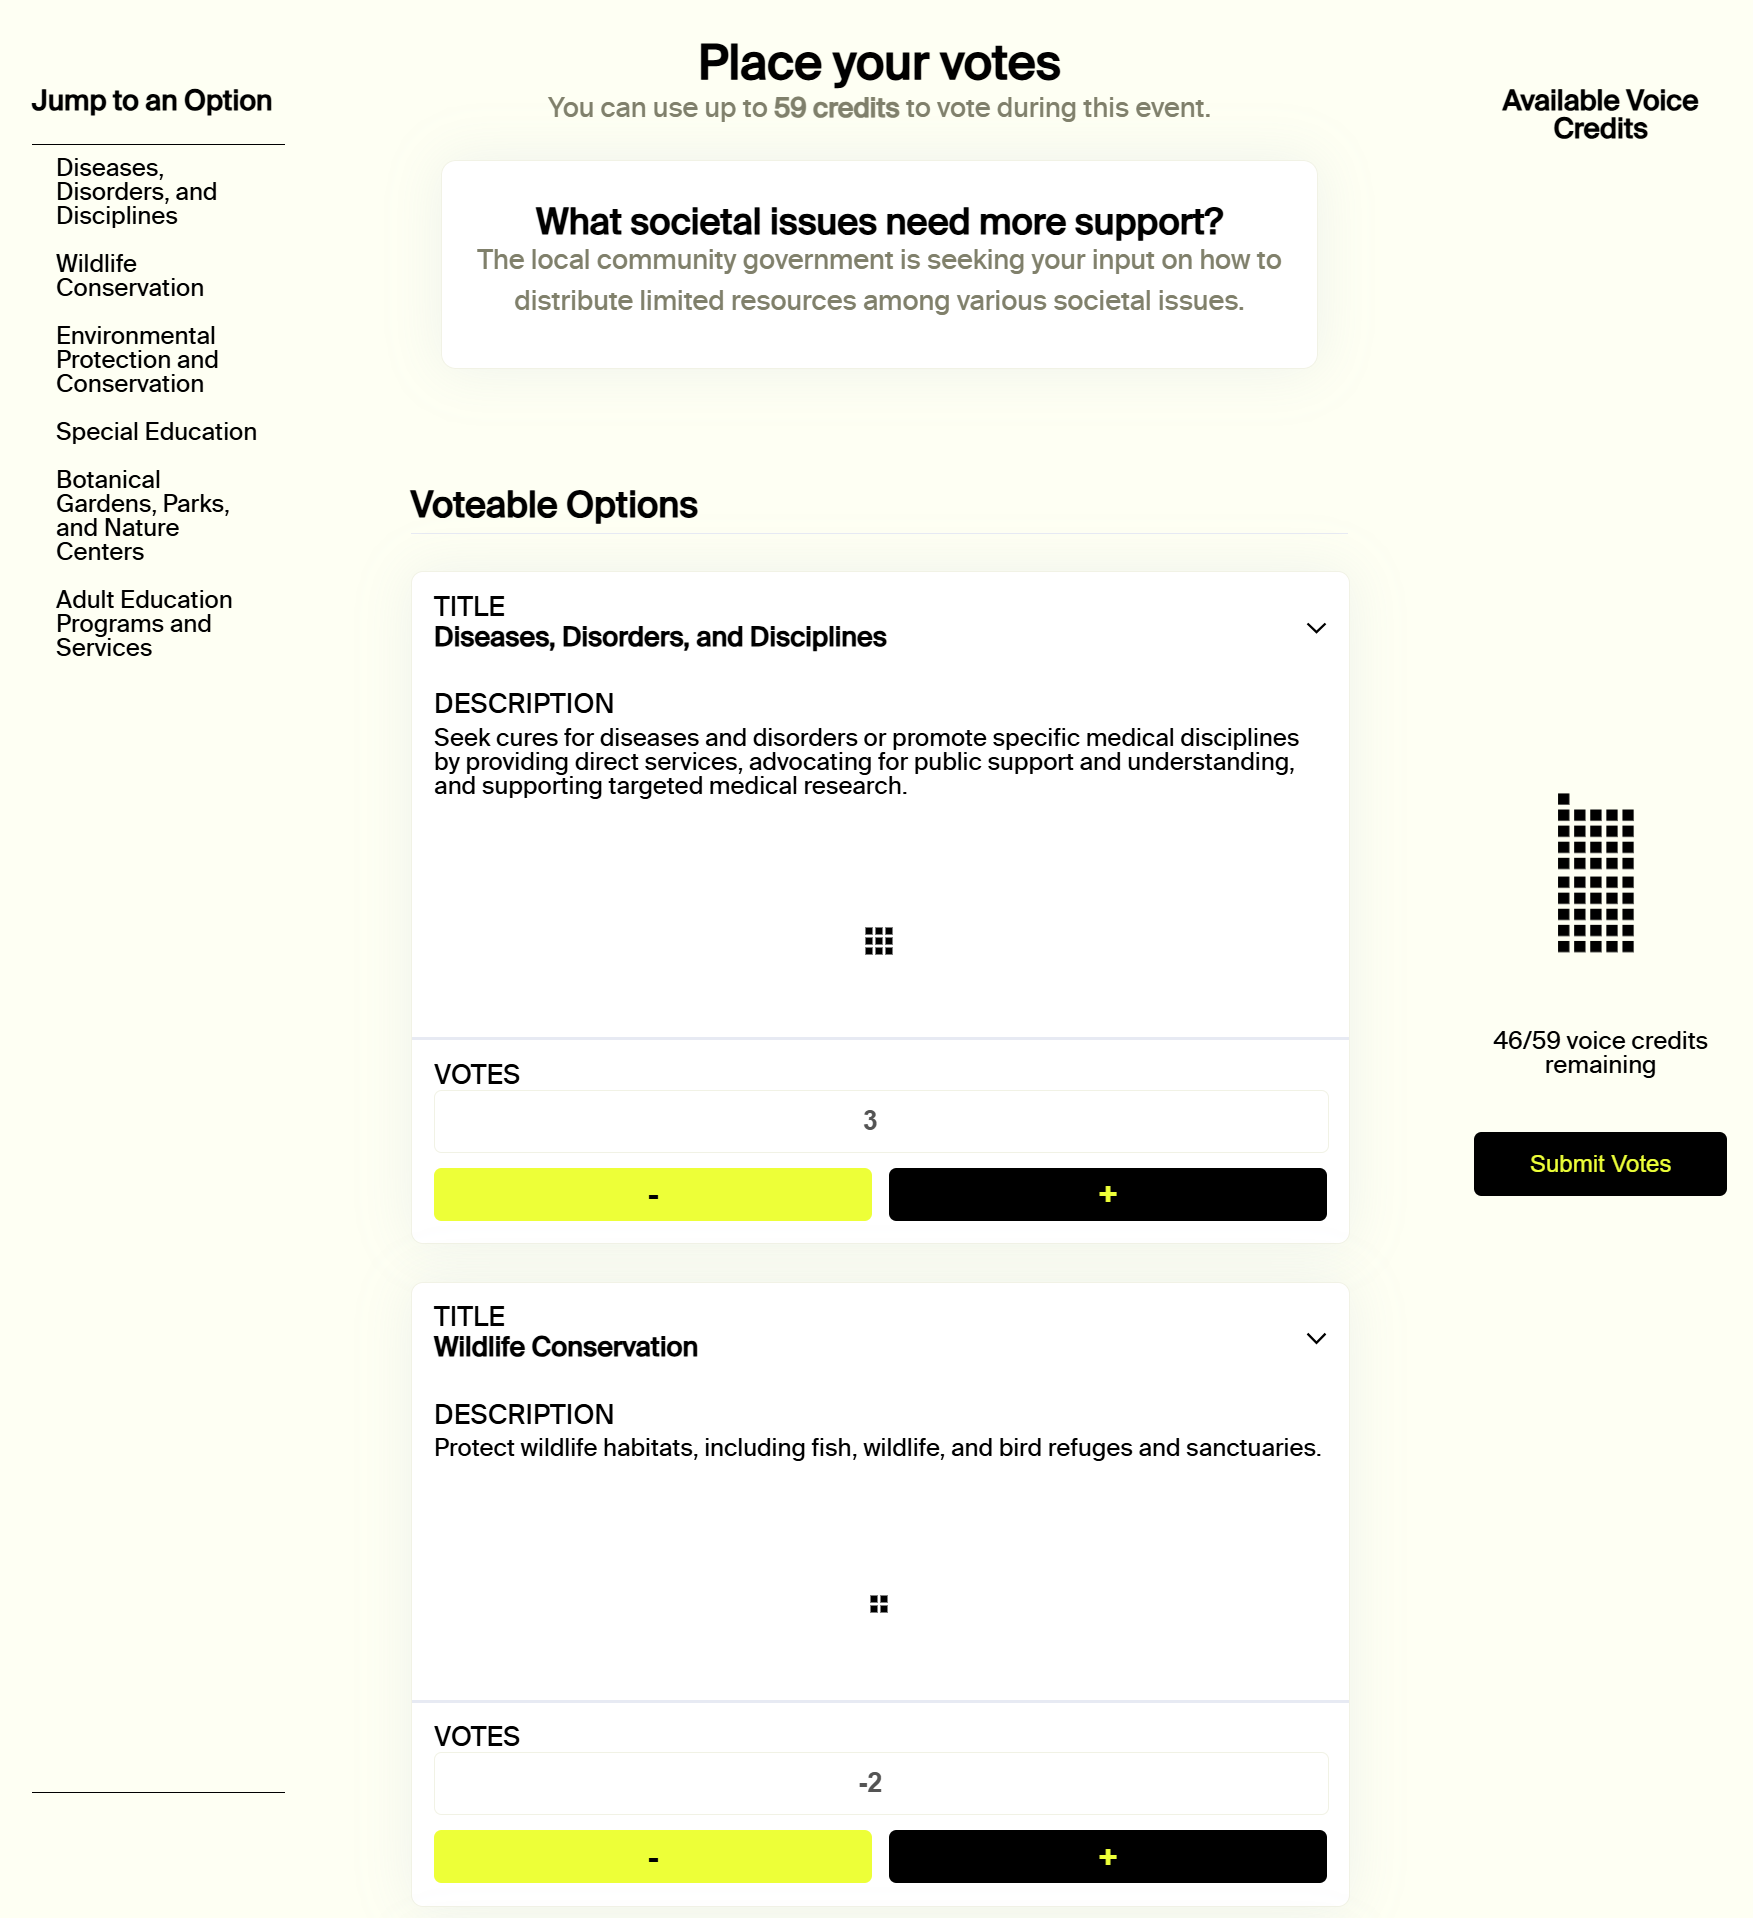
\includegraphics[width=0.72\textwidth]{content/image/curr_interface/rxc_interface.png}
        \caption{An open-sourced QV interface~\cite{RadicalxChangeQuadraticvoting2024} forked from GitCoin~\cite{ReadWhitepaperGitcoin}, used by the RadicalxChange community~\cite{RxC}. This interface presents total credits as small blocks. Votes are updated using plus and minus buttons, with numerical counts shown under each option and surface area as costs.}
        \label{fig:rxcvotingInterface}
    \end{subfigure}
    
    \vspace{0.12cm}
    
    \begin{subfigure}[b]{0.47\textwidth}
        \centering
        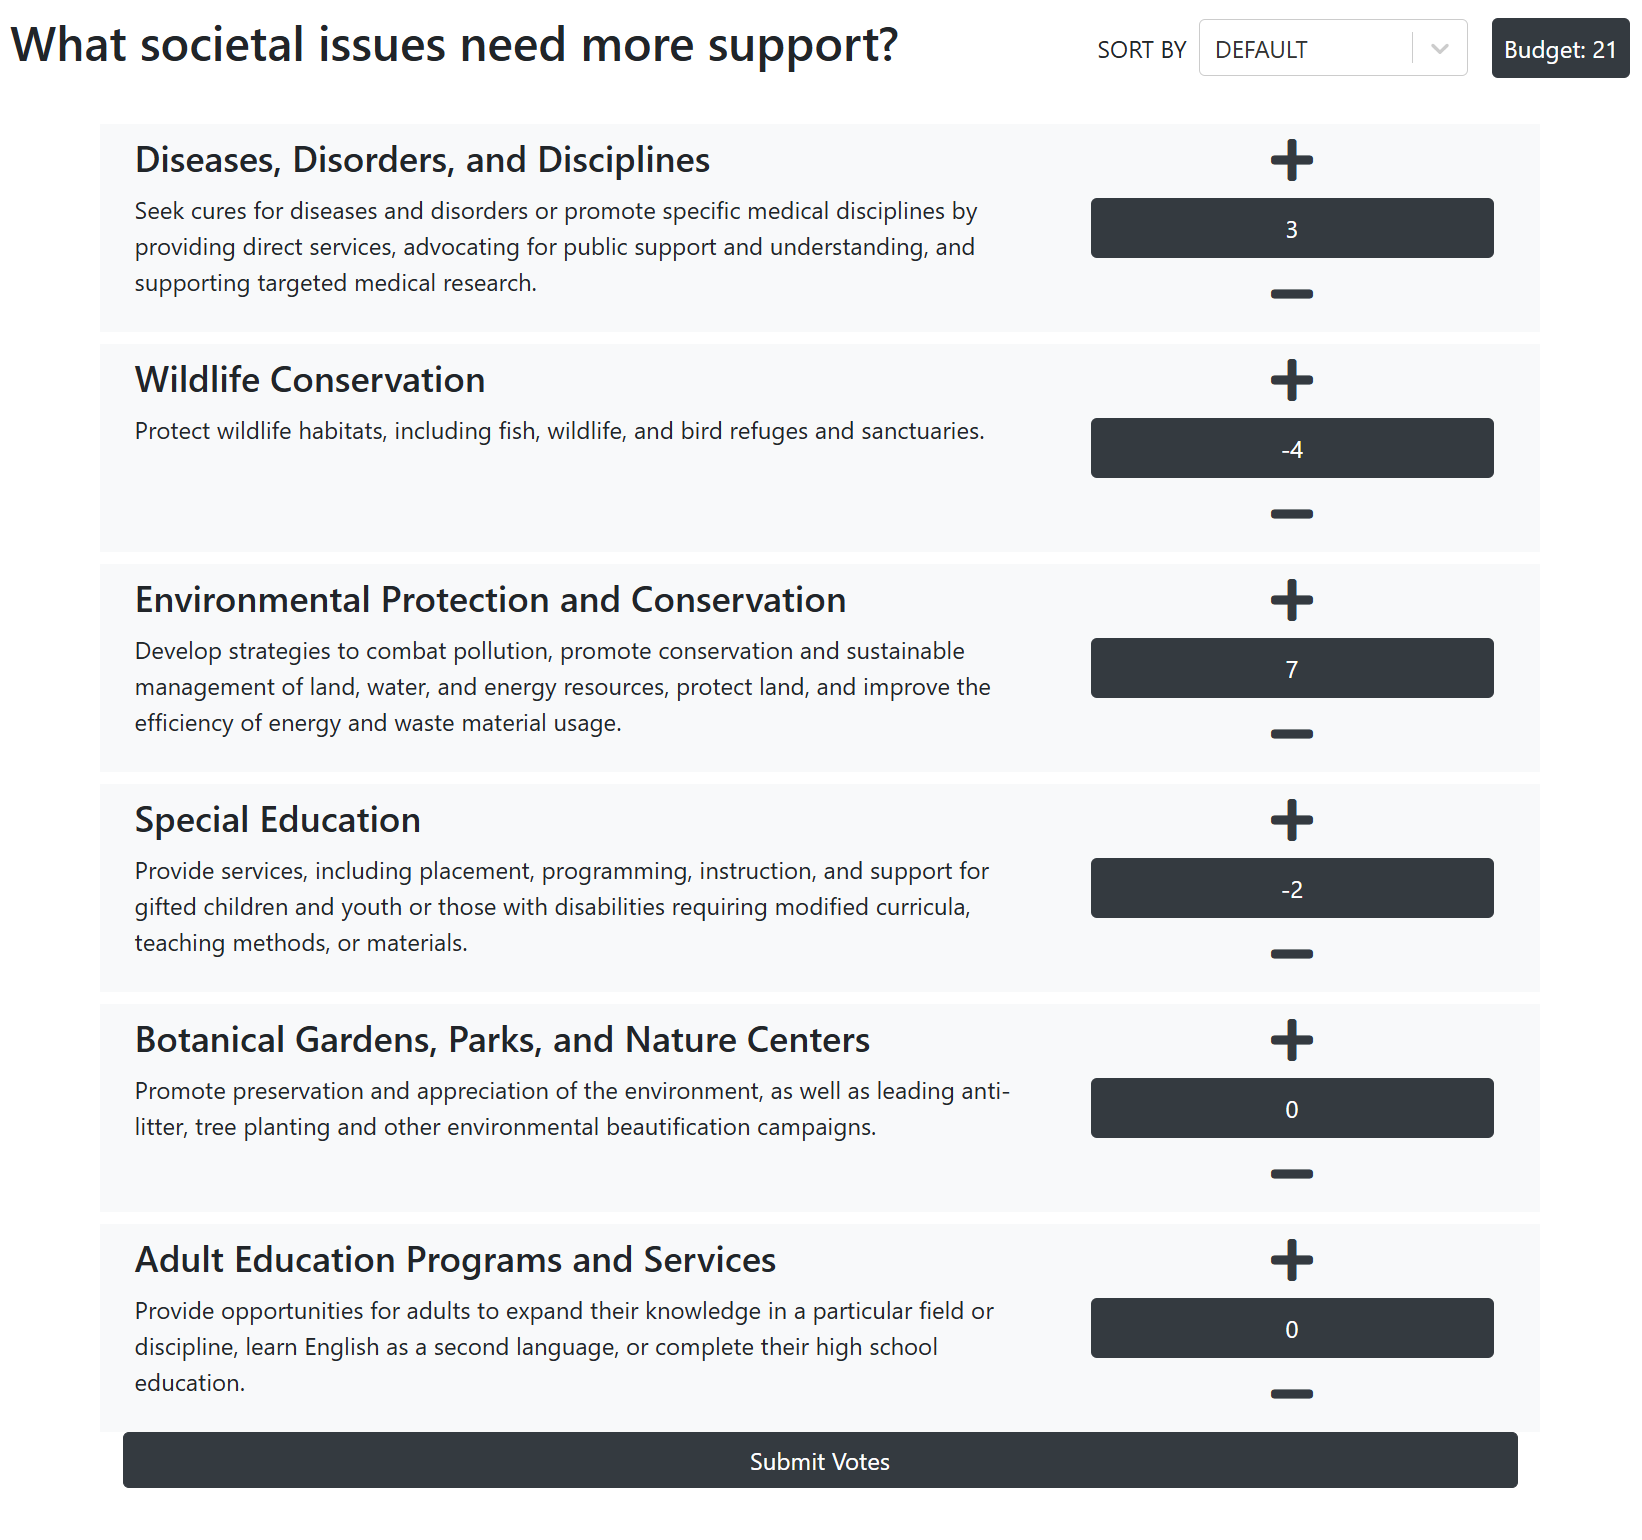
\includegraphics[width=0.72\textwidth]{content/image/curr_interface/geek.sg_interface.png}
        \caption{An open-source QV interface~\cite{yehjxraymondYehjxraymondQvapp2024} offers a publicly available service. Options show only the current number of votes, with credits displayed in the top right corner. This interface does not show the costs of votes but supports sorting options.}
        \label{fig:yehInterface}
    \end{subfigure}
    \hspace{0.4cm}
    \begin{subfigure}[b]{0.47\textwidth}
        \centering
        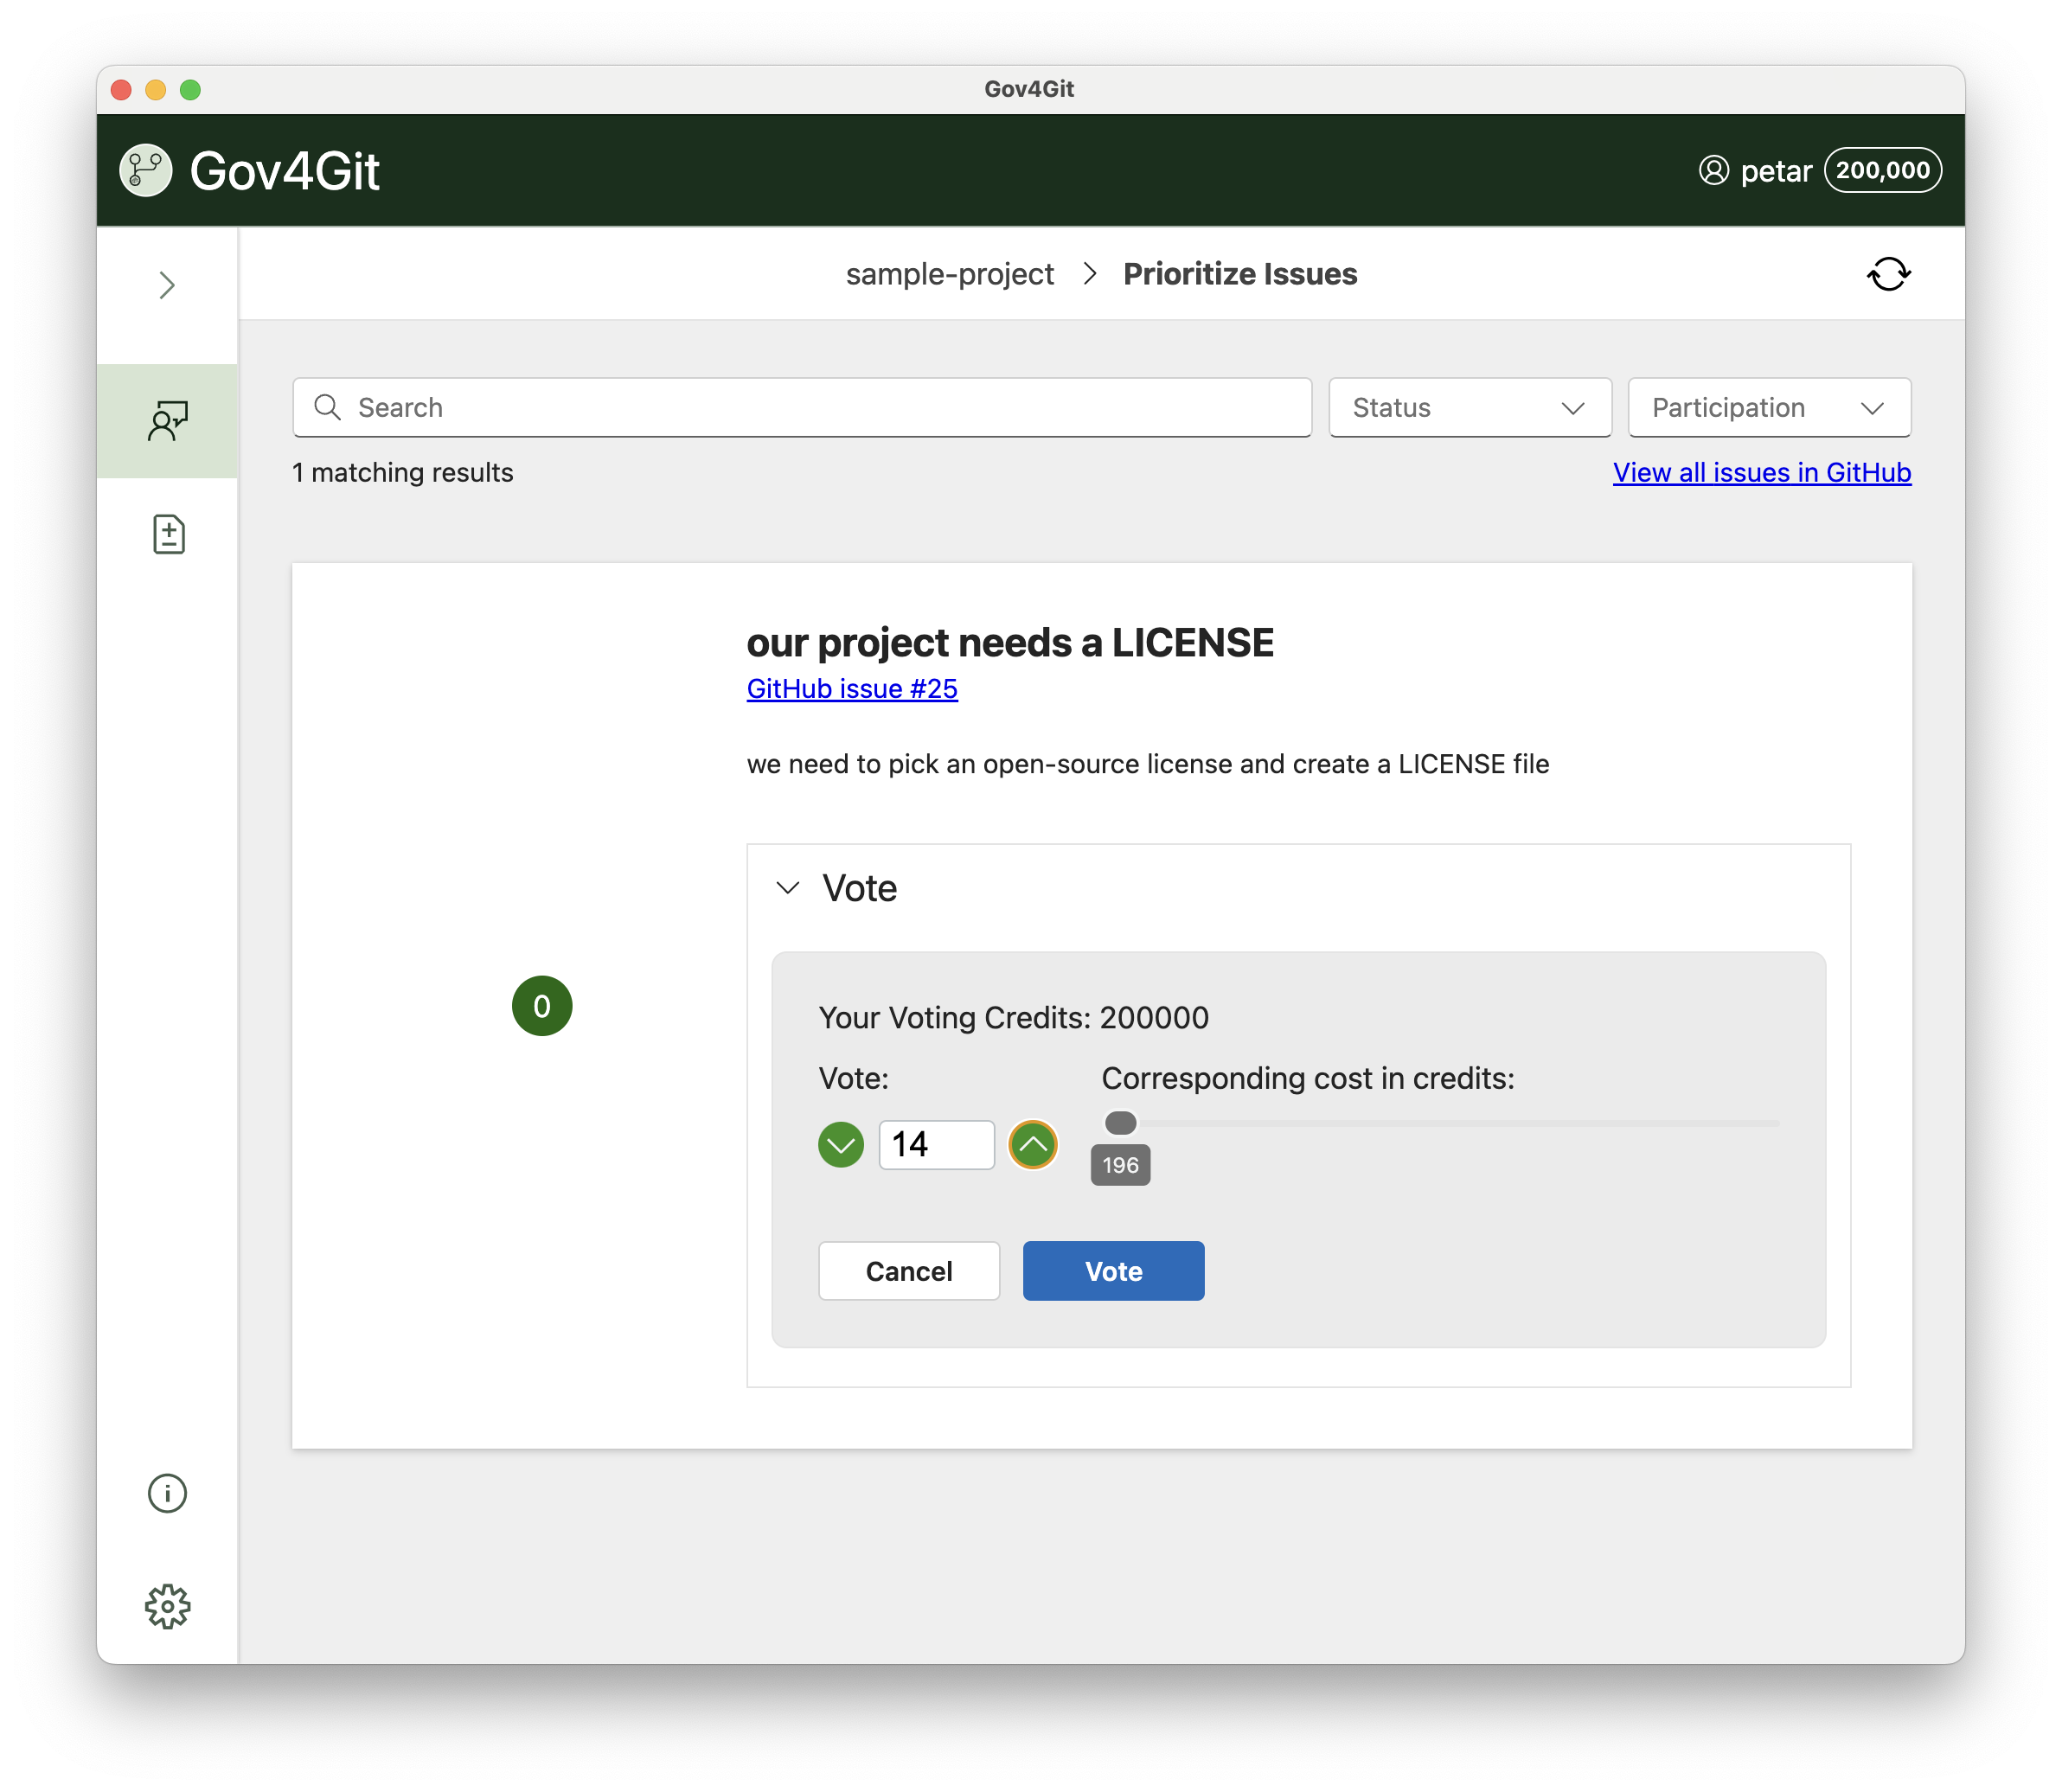
\includegraphics[width=0.72\textwidth]{content/image/curr_interface/appvote.png}
        \caption{The interface designed for gov4git~\cite{Gov4gitDecentralizedPlatform2023} updates votes using arrows under each option, with the associated cost shown as a percentage bar to the right. A search bar exists for searching specific pull requests or issues.}
        \label{fig:gov4gitInterface}
    \end{subfigure}
    
    \vspace{0.15cm}
    
    \begin{subfigure}[b]{0.7\textwidth}
        \centering
        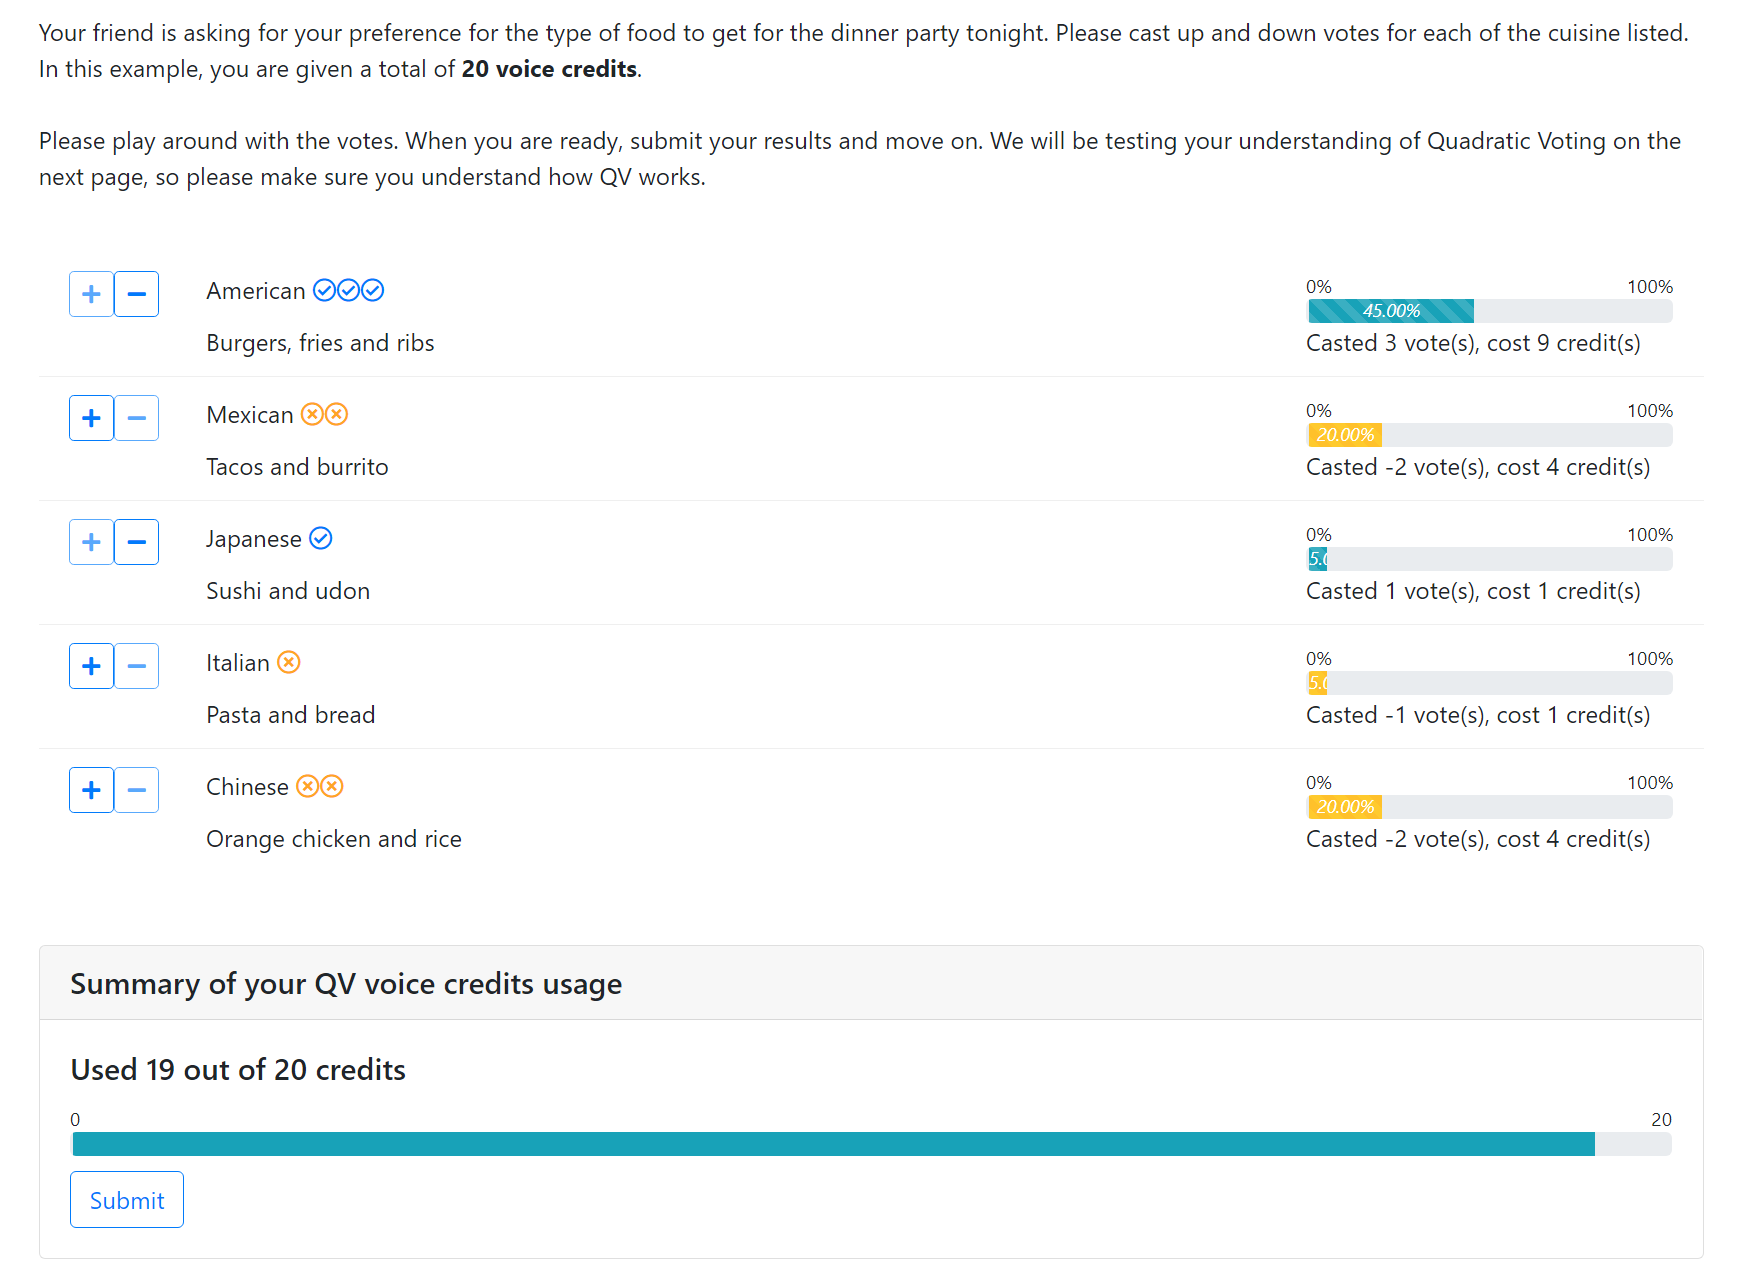
\includegraphics[width=0.50\textwidth]{content/image/curr_interface/cheng_qv.png}
        \caption{The interface used in the research by~\textcite{chengCanShowWhat2021} employs the most visual components. Icons depict the current number of votes, with progress bars signifying the current spending.}
        \label{fig:chengInterface}
    \end{subfigure}
    
    \caption{Recent interface for applications using the quadratic mechanism.}
    \label{fig:qv_interface_external}
\end{figure}
\clearpage
}